% generated by scripts/analysis/label_thresholds.ipynb -- do not edit by hand
\begin{figure}[htbp]
\centering
\pgfplotsset{ltstyle/.style={
  width=0.49\textwidth, height=3.9cm,
  xlabel style={font=\scriptsize}, ylabel style={font=\scriptsize},
  tick label style={font=\scriptsize}, title style={font=\small},
  grid=major, grid style={black!10}},
  ltcut/.style={extra x ticks={#1}, extra x tick labels={},
    extra x tick style={grid=major, major grid style={dashed, black!70}, major tick length=0pt}}}
\definecolor{ltneg}{RGB}{178,68,58}
\definecolor{ltmid}{RGB}{154,154,154}
\definecolor{ltpos}{RGB}{47,125,79}
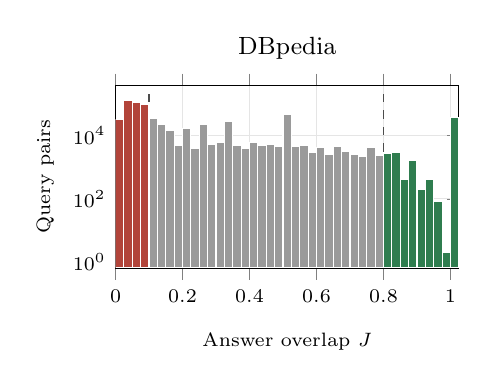
\begin{tikzpicture}
\begin{axis}[ltstyle, title={DBpedia}, ylabel={Query pairs},
  ymode=log, log origin=infty, xmin=0, xmax=1.025, ybar, bar width=0.025, bar shift=0pt,
  xlabel={Answer overlap $J$}, xtick={0,0.2,0.4,0.6,0.8,1}, ltcut={0.1,0.8}]
\addplot[fill=ltneg, draw=white] coordinates {(0.0125,32425) (0.0375,125296) (0.0625,109013) (0.0875,97914)};
\addplot[fill=ltmid, draw=white] coordinates {(0.1125,34727) (0.1375,22775) (0.1625,14466) (0.1875,4960) (0.2125,16403) (0.2375,3879) (0.2625,22540) (0.2875,5050) (0.3125,6089) (0.3375,26771) (0.3625,4771) (0.3875,4025) (0.4125,6115) (0.4375,4835) (0.4625,5270) (0.4875,4386) (0.5125,45250) (0.5375,4615) (0.5625,4925) (0.5875,2873) (0.6125,4204) (0.6375,2586) (0.6625,4350) (0.6875,3068) (0.7125,2541) (0.7375,2207) (0.7625,4135) (0.7875,2293)};
\addplot[fill=ltpos, draw=white] coordinates {(0.8125,2790) (0.8375,2927) (0.8625,422) (0.8875,1619) (0.9125,200) (0.9375,424) (0.9625,83) (0.9875,2) (1.0125,37725)};

\end{axis}
\end{tikzpicture}\hfill
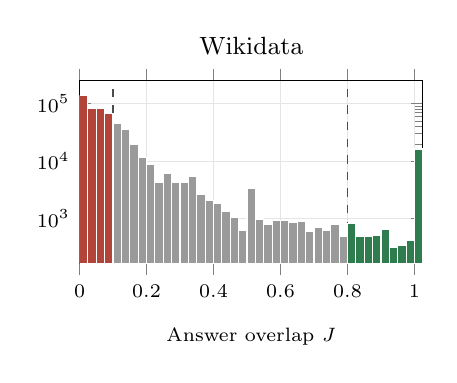
\begin{tikzpicture}
\begin{axis}[ltstyle, title={Wikidata}, ylabel={},
  ymode=log, log origin=infty, xmin=0, xmax=1.025, ybar, bar width=0.025, bar shift=0pt,
  xlabel={Answer overlap $J$}, xtick={0,0.2,0.4,0.6,0.8,1}, ltcut={0.1,0.8}]
\addplot[fill=ltneg, draw=white] coordinates {(0.0125,136785) (0.0375,82823) (0.0625,83023) (0.0875,67764)};
\addplot[fill=ltmid, draw=white] coordinates {(0.1125,44553) (0.1375,35527) (0.1625,19699) (0.1875,11678) (0.2125,8732) (0.2375,4198) (0.2625,6167) (0.2875,4320) (0.3125,4231) (0.3375,5422) (0.3625,2650) (0.3875,2092) (0.4125,1807) (0.4375,1336) (0.4625,1028) (0.4875,630) (0.5125,3289) (0.5375,982) (0.5625,803) (0.5875,939) (0.6125,933) (0.6375,850) (0.6625,887) (0.6875,599) (0.7125,708) (0.7375,634) (0.7625,784) (0.7875,483)};
\addplot[fill=ltpos, draw=white] coordinates {(0.8125,835) (0.8375,481) (0.8625,492) (0.8875,499) (0.9125,646) (0.9375,309) (0.9625,339) (0.9875,416) (1.0125,16226)};

\end{axis}
\end{tikzpicture}

\vspace{2pt}
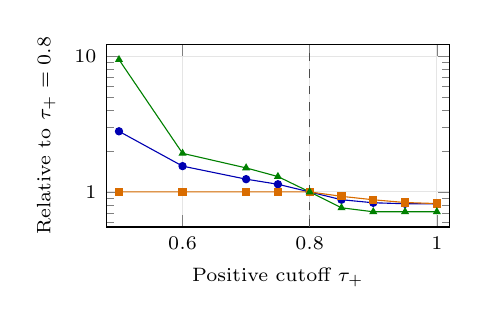
\begin{tikzpicture}
\begin{axis}[ltstyle, title={}, ylabel={Relative to $\tau_+=0.8$}, ymode=log, log ticks with fixed point, legend to name=ltlegend, legend columns=3, legend style={font=\scriptsize, draw=none, /tikz/every even column/.append style={column sep=8pt}},
  xmin=0.48, xmax=1.02, xlabel={Positive cutoff $\tau_+$}, ltcut={0.8}]
\addplot[color=blue!70!black, mark=*, mark size=1.3pt] coordinates {(0.5000,2.79787) (0.6000,1.54953) (0.7000,1.24195) (0.7500,1.13916) (0.8000,1) (0.8500,0.876234) (0.9000,0.832049) (0.9500,0.81854) (1.0000,0.8167)};
\addlegendentry{positive pairs}
\addplot[color=orange!85!black, mark=square*, mark size=1.3pt] coordinates {(0.5000,1.00171) (0.6000,1.00128) (0.7000,1.00043) (0.7500,1.00043) (0.8000,1) (0.8500,0.928327) (0.9000,0.875267) (0.9500,0.835687) (1.0000,0.82071)};
\addlegendentry{queries with a positive}
\addplot[color=green!50!black, mark=triangle*, mark size=1.3pt] coordinates {(0.5000,9.44099) (0.6000,1.92547) (0.7000,1.50311) (0.7500,1.29814) (0.8000,1) (0.8500,0.763975) (0.9000,0.714286) (0.9500,0.714286) (1.0000,0.714286)};
\addlegendentry{largest positive component}
\end{axis}
\end{tikzpicture}\hfill
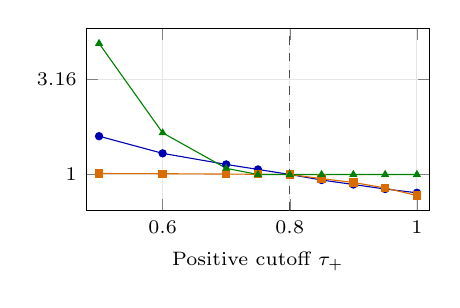
\begin{tikzpicture}
\begin{axis}[ltstyle, title={}, ylabel={}, ymode=log, log ticks with fixed point, 
  xmin=0.48, xmax=1.02, xlabel={Positive cutoff $\tau_+$}, ltcut={0.8}]
\addplot[color=blue!70!black, mark=*, mark size=1.3pt] coordinates {(0.5000,1.58741) (0.6000,1.29037) (0.7000,1.12888) (0.7500,1.06259) (0.8000,1) (0.8500,0.93499) (0.9000,0.886035) (0.9500,0.838858) (1.0000,0.801561)};
\addplot[color=orange!85!black, mark=square*, mark size=1.3pt] coordinates {(0.5000,1.01152) (0.6000,1.00903) (0.7000,1.00475) (0.7500,1.00214) (0.8000,1) (0.8500,0.950938) (0.9000,0.907698) (0.9500,0.850202) (1.0000,0.775125)};
\addplot[color=green!50!black, mark=triangle*, mark size=1.3pt] coordinates {(0.5000,4.86538) (0.6000,1.65385) (0.7000,1.07692) (0.7500,1) (0.8000,1) (0.8500,1) (0.9000,1) (0.9500,1) (1.0000,1)};
\end{axis}
\end{tikzpicture}

\vspace{1pt}
\ref{ltlegend}
\caption{Label thresholds. Top: answer overlap $J$ of all query pairs with $J>0$ (log scale), colored
by label: negative ($J\leq0.1$), unlabeled, positive ($J\geq0.8$; the last bar is $J=1$).
Bottom: positive pairs, queries with at least one positive, and the largest positive component
for other positive cutoffs $\tau_+$, relative to $\tau_+=0.8$ (log scale). Counts are over all pairs of the retained queries.}
\label{fig:labelthresholds}
\end{figure}
